\documentclass[10pt,fleqn]{beamer}

\usecolortheme{crane}
\usepackage{bm}
\usepackage{color}
\usepackage{amsmath,amssymb,amsfonts,latexsym}

\usepackage[spanish]{babel}
\usepackage[utf8]{inputenc}
\usepackage[T1]{fontenc}
\usepackage{listings}

\usepackage{xcolor}

\definecolor{aliceblue}{rgb}{0.94, 0.97, 1.0}
\definecolor{beige}{rgb}{0.96, 0.96, 0.86}
\definecolor{blanco}{rgb}{1, 1, 1}
\definecolor{almond}{rgb}{0.94, 0.87, 0.8}
\definecolor{lightgray}{gray}{0.9}
\definecolor{dkgreen}{rgb}{0,0.6,0}
\definecolor{gray}{rgb}{0.5,0.5,0.5}


\lstdefinestyle{customc}{
  belowcaptionskip=1\baselineskip,
  breaklines=true,
  frame=L,
  xleftmargin=\parindent,
  language=C,
  showstringspaces=false,
  basicstyle=\footnotesize\ttfamily,
  keywordstyle=\bfseries\color{green!40!black},
  commentstyle=\itshape\color{purple!40!black},
  identifierstyle=\color{blue},
  stringstyle=\color{orange},
}

\lstdefinestyle{customasm}{
  belowcaptionskip=1\baselineskip,
  frame=L,
  xleftmargin=\parindent,
  language=[x86masm]Assembler,
  basicstyle=\footnotesize\ttfamily,
  commentstyle=\itshape\color{purple!40!black},
}

\lstset{escapechar=@,style=customc}


% Incluir figuras .pdf, .png, .jpg, .gif, .eps, etc. SIN extensi\’on
%\usepackage{epstopdf}
%\DeclareGraphicsExtensions{.pdf,.png,.jpg,.gif, .eps}
\usefonttheme{professionalfonts} % fuentes de LaTeX

% tema escogido en este ejemplo
\setbeamercovered{transparent}

\begin{document}

{
\usebackgroundtemplate{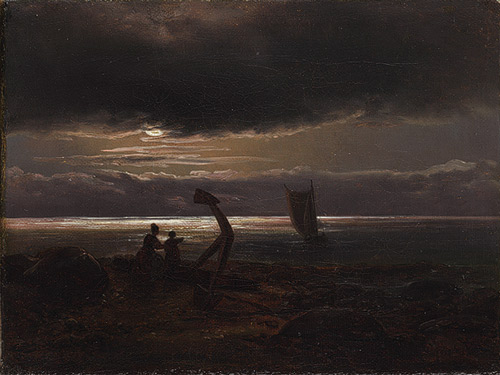
\includegraphics[width= \paperwidth, height=\paperheight]{portada.jpg}}


\title{  \textcolor{blanco}{Cifrado Parcial}       \\}
\subtitle{    \textcolor{beige}{Conceptos y algoritmo}          }

\author{   {\bf  \textcolor{aliceblue}{Marcos Daniel C. Calderón}    }    \\ 
\vspace*{0.5cm}}
\date{   \textcolor{almond}{2014}     }
\frame{\titlepage}
}




\section{Fundamentos.}

\begin{frame}
\begin{block}{Definición.}
El cifrado parcial consiste en fragmentar la información en pequeños pedazos, después, se aplica un método de  cifrado a cada una de las partes obtenidas. 
\end{block}
\end{frame}


\begin{frame}
\frametitle{Ventajas del cifrado Parcial}
\begin{itemize}
\item Reducción del tiempo de procesamiento.
\item Reducción del ancho de banda requerido.
\item Muy útil para esquemas de cifrado de video e imágemes.
\end{itemize}
\end{frame}





{
\setbeamercolor{background canvas}{bg=black}

\begin{frame}
\frametitle{   Parte 1. Permutación de segmentos.   }
\begin{figure}[H]
\centering
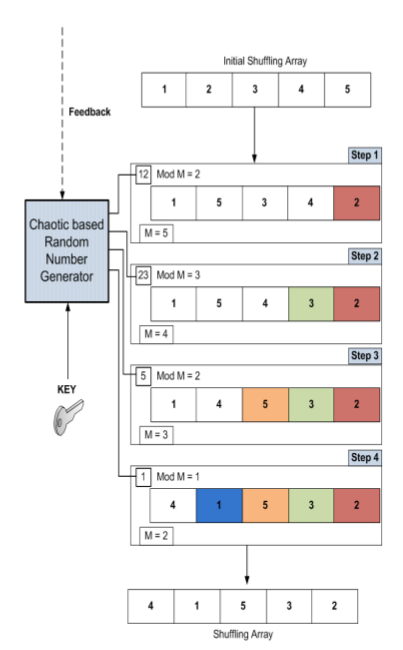
\includegraphics[width=4cm]{logos/per.png}
\end{figure}
\end{frame}
}



\begin{frame}[fragile]
\frametitle{Parte 1. Un código para permutación...  }


\begin{lstlisting}
/*========= Proceso de Permutacion ==================*/
srand (time(NULL));
M=10;
for(iSeg =1; iSeg < Lsegmentos; iSeg++){
M=M-1;
R= rand(); //Generate random number R
T= R%M;
		
/*Ahora, hacemos el intercambio que sea necesario.*/
for(iTamSeg=0; iTamSeg<tamSegmento; iTamSeg++){
  pos1=(tamSeg*(T)+iTamSeg) + (irtp*tamRTP);
  pos2=(tamSeg*(M)+iTamSeg) + (irtp*tamRTP);
  auxiliar = datosArchivo[pos1];
  datosArchivo[pos1]=datosArchivo[pos2];
  datosArchivo[pos2]= auxiliar;
	        }
	}
/*===================================================*/
			
\end{lstlisting}
\end{frame}





\begin{frame}[fragile]
\frametitle{Parte 1. Resultados  }

A continuación se muestra un ejemplo sencillo de los segmentos que se van a intercambiar en un paquete RTP que fué dividido en 10 segmentos.


\begin{lstlisting}
 El paquente numero  1:
 "Resultados similares"
 
 El paquente numero  2:
 T: 8    M: 9  
 T: 2    M: 8   
 T: 5    M: 7
 T: 3    M: 6   
 T: 4    M: 5  
 T: 1    M: 4   
 T: 1    M: 3   
 T: 1    M: 2   
 T: 0    M: 1   
\end{lstlisting}
\end{frame}




\begin{frame}[fragile]
\frametitle{Parte 1. Recomendaciones para el proceso de permutación.  }

\begin{itemize}
\item Asegurarse que siempre haya intercambio. (T debe ser distinto de M en el esquema presentado).

\item Justo antes de ejecutar el intercambio, aplicar el proceso de inversión de bits.

\end{itemize}

\end{frame}





{
\setbeamercolor{background canvas}{bg=black}
\begin{frame}
\frametitle{   Parte 2. Inversión de Bits. Criterio 1.   }

\begin{itemize}
\item  \textcolor{beige}{¿Qué pasa si el bit de referencia queda en un extremo? 
Mejor aseguarse SIEMPRE que la referencia no quede en un extremo para que de y db estén bien definidos.} 



\end{itemize}

\begin{figure}[H]
\centering
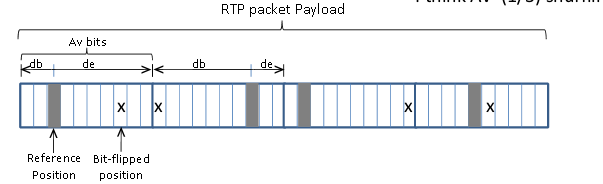
\includegraphics[width=8cm]{logos/es1.png}
\end{figure}
\end{frame}
}





{
\setbeamercolor{background canvas}{bg=black}
\begin{frame}
\frametitle{   Parte 2. Inversión de Bits. Criterio 2. }

\begin{itemize}
\item 

\textcolor{beige}{ En este caso, el bit de referencia será aquel que se haya invertido en una iteración anterior. (Con este esquema se evitan huecos).} 






\end{itemize}

\begin{figure}[H]
\centering
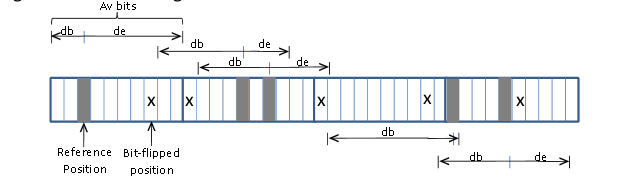
\includegraphics[width=8cm]{logos/es2.png}
\end{figure}
\end{frame}
}



\begin{frame}[fragile]
\frametitle{Parte 2. Inversión de bits hasta el momento.  }

La inversión de bits en este momento consta de los siguientes pasos:


\begin{itemize}
\item Supongamos (como ocurre en el programa actual), que el tamaño del segmento \textbf{a intercambiar} es de 20 bytes (160 bits), entonces dividimos entre 32 bits, para obtener un total de 5 iteraciones. 

\item Ahora, para cada una de las 5 iteraciones, un apuntador se mueve a lo largo del segmento cada 4 bytes (32 bits) y se aplica la inversión de bits de acuerdo a los criterios mencionados.

\begin{lstlisting}
p = IC_int[count]&7;
pos_f+= p;				
if(p&1){
  step = IC_int[count+1]%p;
  pos_f -= step;
}
else{
  step = IC_int[count+1]%(BlockSize - p);
  pos_f += step;
}
Pack_temp[pos_byte + (pos_f/8)]^= 1<<(8 - (pos_f&7));			
\end{lstlisting}


\end{itemize}

\end{frame}









\section{Desarrollo del algoritmo de cifrado parcial.}





\section{Mapas caóticos.}

\begin{frame}[fragile]
\frametitle{Utilización de mapas caóticos acoplados.  Un ejemplo...  }

\begin{itemize}

\item A continuación, se muestra un conjunto de cuatro mapas acoplados donde se utiliza un fragmento de texto plano.
\begin{lstlisting}
for(jj=0; jj<4; jj++){
	hh+=W_int[jj]^IC_int[jj]^PText[jj];
}
	hh = hh%20;

for(jj=0; jj<4; jj++){
	IC_int[jj] = Renyi_int(IC_int[jj],beta[jj]) + hh;
    PText[jj] = Pack_temp[pos_byte + jj];
}				
\end{lstlisting}

\end{itemize}

\end{frame}




\begin{frame}[fragile]
\frametitle{  Utilización de mapas caóticos acoplados.  Uso del texto plano. }

En el código existente se utilizó el texto plano de la siguiente manera:
\begin{lstlisting}
for(jj=0; jj<4; jj++){
	hh+=W_int[jj]^IC_int[jj]^PText[jj];
}
	hh = hh%20;			
\end{lstlisting}




Pero, puede haber otras alternativas.


\end{frame}



\section{Observaciones finales.}
\begin{frame}[fragile]
\frametitle{  Observaciones finales. }


\begin{itemize}
\item Evitar el uso de memoria auxiliar, (arreglos auxiliares).

\item Evitar operaciones innecesarias (verificar que siempre ocurran tareas significativas).

\end{itemize}

\end{frame}



\end{document}




